\chapter{Extracción de datos}

La fuente de información de donde obtuvimos los datos utilizados son las páginas de los horarios de la Facultad. En la \figurename{~\ref{pagFC}} se muestra un ejemplo de dichas páginas. Cada página contiene toda la posible información de los grupos de una materia, un semestre y una carrera. Cabe mencionar que sólo tomamos en cuenta la información de las carreras del Departamento de Matemáticas, las cuales son: Actuaría, Ciencias de la Computación, Matemáticas y Matemáticas Aplicadas.

\begin{figure}[H]
\centering

\includegraphics[width=\textwidth]{Fuente_de_info} %scale = 0.5
%\url{http://www.fciencias.unam.mx/docencia/horarios/20201/217/607} %%URL de la imagen
\caption[\textit{Página de horarios de la Facultad de Ciencias}]{\textit{Página de horarios de la Facultad de Ciencias: Muestra la información de los horarios de la materia ``Lenguajes de Programación y sus Paradigmas'', de la carrera de Matemáticas, plan 1983, del semestre 2020-1.}}\label{pagFC}
\end{figure}

La información que se puede extraer de las páginas mencionadas es: \textit{nombre de profesores, nombre de ayudantes, salón, horario, plan, carrera, año, número de semestre, materia, semestre de la materia, tipo de materia} e \textit{información de exámenes finales}.


\section{Estructura de las URL's}

Al iniciar la búsqueda de información notamos que las URL's de las páginas web de los horarios de la Facultad tenían una estructura similar. Ésto nos permitió poder realizar la búsqueda de la información de una manera automática y mucho más rápida. Observamos que la estructura que siguen las URL's mencionadas es la siguiente:

\begin{center}
\textit{\textbf{http://www.fciencias.unam.mx/docencia/horarios/a/b/c}}
\end{center}

Se tiene una raíz común para todas las páginas y al final se tienen tres números los cuales representan:

\begin{itemize}
\item[ ] \textit{\textbf{a}} = año y número de semestre

\item[ ] \textit{\textbf{b}} = clave del plan de estudios

\item[ ] \textit{\textbf{c}} = número de materia
\end{itemize}

Para este trabajo tomamos en cuenta sólo los planes de estudio vigentes hasta el semestre 2020-1. Es decir, tomamos todos los planes mostrados en la tabla \tablename{~\ref{PlanesEstudio}}, salvo el plan 1972 de Actuaría (el cual ya no está vigente). Dicha tabla muestra los planes de estudio de cada carrera con su clave correspondiente.

\begin{table}[h]
\centering
\begin{tabular}{|c|c|}
 \hline 
  \textbf{PLAN} & \textbf{CLAVE} \\ 
 \hline 
 \multicolumn{2}{|c|}{Actuaría} \\ 
 \hline 
 1972 & 214 \\ 
 \hline 
 2000 & 119 \\ 
 \hline 
 2006 & 1176 \\ 
 \hline 
 2015 & 2017 \\ 
 \hline 
 \multicolumn{2}{|c|}{Ciencias de la Computación} \\ 
 \hline 
 1994 & 218 \\ 
 \hline 
 2013 & 1556 \\ 
 \hline 
 \multicolumn{2}{|c|}{Matemáticas} \\ 
 \hline 
 1983 & 217 \\ 
 \hline 
 \multicolumn{2}{|c|}{Matemáticas Aplicadas} \\ 
 \hline 
 2017 & 2055 \\ 
 \hline 
 \end{tabular}
\caption[\textit{Planes de estudio por carrera con clave}]{\textit{Planes de estudio por carrera con clave: La clave de cada plan de estudios se sutituye en \textbf{b} en la estructura de las URL's de las páginas de la Facultad.}}\label{PlanesEstudio}
\end{table}

Una vez identificada la estructura de las URL's pudimos realizar la búsqueda de información de manera automatizada. Originalmente decidimos que $c \in \{1,2,3, \ldots, 10 000\}$. Después hicimos una función que genera una matriz llamada \textit{mat\_posibles\_url}. La función sólo guarda las URL's que si existen. La descripción de lo que contiene cada columna de la matriz \textit{mat\_posibles\_url} la podemos ver en la \tablename{~\ref{matPosiblesURL}}. Finalmente al obtener dicha matriz, observamos que el valor máximo que toma $c$ es 991, por lo que redujimos su conjunto de posibles valores y definimos $c \in \{1, \ldots, 1 000\}$.

\dfNmatrizChica %%Tabla con la información de la matriz chica

Decidimos buscar información en 25 semestres, del 2008-1 al 2020-1. Al multiplicar el número de semestres por los posibles valores de \textbf{c} $(25 \times \textbf{c})$ obtuvimos un número cercano a $25,000$. Este valor es una aproximación del número de posibles URL's con información de los horarios de la Facultad. Notemos que no estamos contando los planes de estudio, de ser así el número supera las $170,000$ posibles URL's. Deseamos obtener información de cada una de esas páginas. Obtener dicha información ingresando a cada una de las páginas es complicado por lo que es necesario hacerlo de manera automatizada. Para extraer los datos de las páginas de la Facultad utilizamos una aplicación de \textit{Google Chrome} llamada \textit{SelectorGadget}. La cual explicamos en la siguiente sección.

\section{Extracción de datos con la aplicación SelectorGadget}

La aplicación \textit{SelectorGadget} permite seleccionar la información deseada y arroja una sección del código CSS de una página web. Dicho código se introduce en \textit{R} para poder seleccionar y descargar la información deseada. A continuación veremos los pasos que se deben de seguir para obtener el código CSS de la información seleccionada. Los colores y señalizaciones mencionados hacen referencia a la \figurename{~\ref{appSelectorGadget}}. En dicha figura podemos ver un ejemplo del funcionamiento de la aplicación.

\begin{enumerate}
\item Presionar el ícono de la aplicación, el cual es una lupa (señalado por la flecha roja).

\item Seleccionar la información deseada (en color verde).

\item La aplicación automáticamente selecciona todas las entradas que coindiciden (en color amarillo).

\item En caso de que se haya seleccionado más información de la deseada entonces dar click sobre la información excedente (en color rojo).

\item  En el cuadro de texto, la aplicación arroja la sección del código CSS correspondiente a la información seleccionada. También muestra el número de entradas selecionadas (en óvalos rojos).
\end{enumerate}


\begin{figure}[h]
\centering
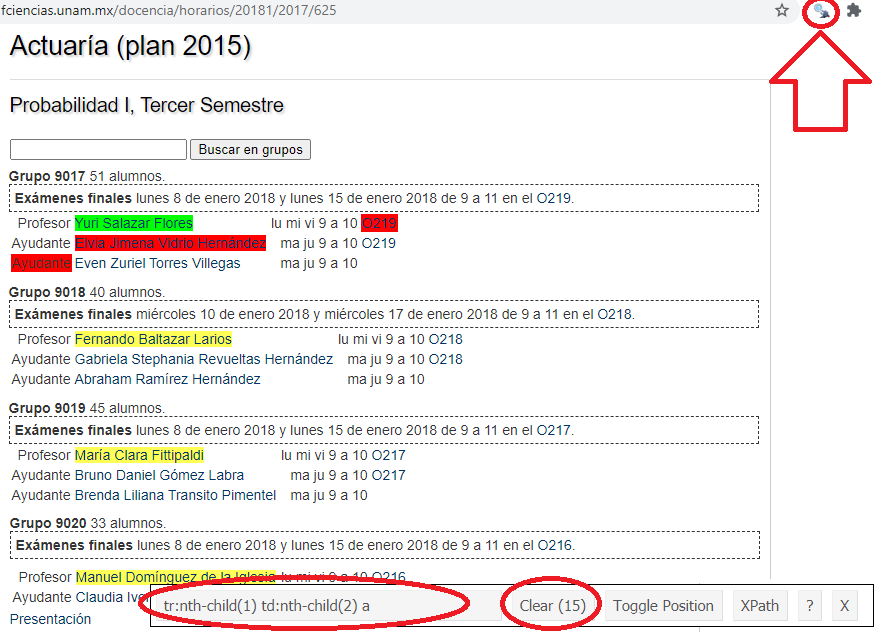
\includegraphics[width=\textwidth]{SelectorGadget} %scale = 0.65
%\url{http://www.fciencias.unam.mx/docencia/horarios/20181/2017/625} %%URL de la imagen
\caption[\textit{Aplicación SelectorGadget}]{\textit{Aplicación SelectorGadget: Se muestra cómo se ve una página con los horarios de la Facultad al usar la aplicación mientras se selecciona la información que deseamos extraer.}}\label{appSelectorGadget}
\end{figure}

En el ejemplo mostrado en la \figurename{~\ref{appSelectorGadget}},se seleccionaron 15 entradas correspondientes a los nombres de los profesores en una página con la información de la materia \textit{Probabilidad I}, en el plan 2015 de Actuaría. Los pasos a seguir son los mismos sin importar la información que se desea obtener, lo único que cambia es el código CSS que arroja la aplicación.


\section{Tipos de grupos de las páginas web de la Facultad de Ciencias} \label{TiposDeGpos}

Al inicio encontramos tres tipos de grupos dentro de las páginas de horarios de la Facultad. Cada uno con información similar, pero hicimos la separación de acuerdo a sus diferencias. Cabe mencionar que en este trabajo consideramos como semestre actual al semestre $2020-1$. En todos los grupos se puede encontrar la información del nombre de profesor, nombre del o de los ayudantes, salón, horario y el número de alumnos inscritos en el grupo.

\begin{enumerate}
\item[a)] En el grupo \textbf{A} se tienen las páginas correspondientes al semestre actual. Este grupo tiene la información del número de lugares diponibles por salón, pero no contiene la información de los exámenes finales, porque se considera que el semestres aún está en curso y aún no termina. En la \figurename{~\ref{GpoA}} podemos ver un ejemplo de este tipo de grupo.

\begin{figure}[H]
\centering
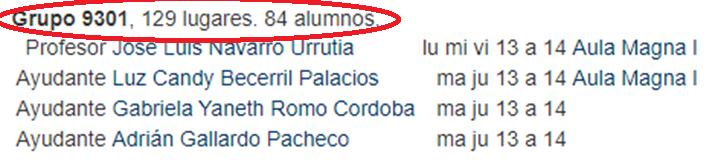
\includegraphics[scale = 0.8]{GrupoA} %width=\textwidth
%\url{http://www.fciencias.unam.mx/docencia/horarios/20201/2017/1707}
\caption[\textit{Tipo de grupo A}]{\textit{Tipo de grupo A: Correspondiente al semestre en curso que aún no finaliza.}}\label{GpoA}
\end{figure}


\item[b)] En el grupo \textbf{B} se tienen las páginas correspondientes a semestres entre el $2018-2$ y el semestre anterior al actual, con respecto al año en curso. En este tipo de grupos se tiene información del número de lugares disponibles por salón y la información de los exámenes finales, porque son semestres que ya finalizaron. En la figura \figurename{~\ref{GpoB}} encontramos un ejemplo de este tipo de grupo.

\begin{figure}[H]
\centering

\includegraphics[scale = 0.8]{GrupoB} %width=\textwidth
%\url{http://www.fciencias.unam.mx/docencia/horarios/20182/217/625}
\caption[\textit{Tipo de grupo B}]{\textit{Tipo de grupo B: Correspondiente a semestres ya finalizados, posteriores al semestre 2018-2.}}\label{GpoB}
\end{figure}

\item[c)] En el grupo \textbf{C} se tienen las páginas correspondientes a semestres anteriores al $2018-1$, incluyéndolo. Este tipo de grupos tiene información de los exámenes finales, pero no contiene la información del número de lugares disponibles por salón. En la figura \figurename{~\ref{GpoC}} podemos ver un ejemplo.

\begin{figure}[H]
\centering
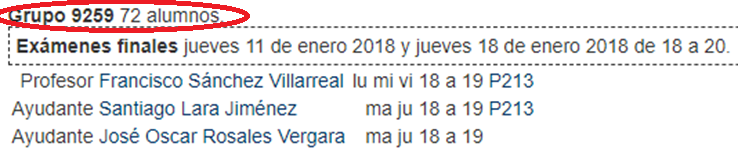
\includegraphics[scale = 0.8]{GrupoC} %width=\textwidth
%\url{http://www.fciencias.unam.mx/docencia/horarios/20181/1556/399}
\caption[\textit{Tipo de grupo C}]{\textit{Tipo de grupo C: Correspondiente a semestres ya finalizados, anteriores al semestre 2018-1, incluyéndolo.}}\label{GpoC}
\end{figure}
\end{enumerate}


\section{Limpieza de base de datos}

Se puede encontrar que, en general, cuando uno realiza la limpieza de datos se hace el 80\% del análisis de los datos. Es en ese momento en donde se encuentran los diferentes problemas que se pueden presentar. Se pueden encontrar posibles errores en los datos, información incompleta, o valores poco comunes de acuerdo al comportamiento observado. Los problemas que encontramos al limpiar los datos se desglosan en las siguientes subsecciones.

\subsection{Problemas de falta de información}

Encontramos diferentes tipos de páginas que tenían grupos sin información e incluso páginas sin información alguna. Para guardar la información consideramos sólo los grupos que al menos tenían: nombre de profesor, número de alumnos inscritos y horario. A continuación se muestran varios ejemplos con los diferentes casos encontrados. %con falta de información.


\begin{itemize}
\item[-] En la figura \ref{pagEnBlanco} vemos un ejemplo de páginas en las cuales se tiene el nombre de la materia, pero no hay información de algún grupo: \url{http://www.fciencias.unam.mx/docencia/horarios/20081/1556/803}

\begin{figure}[H]
\centering
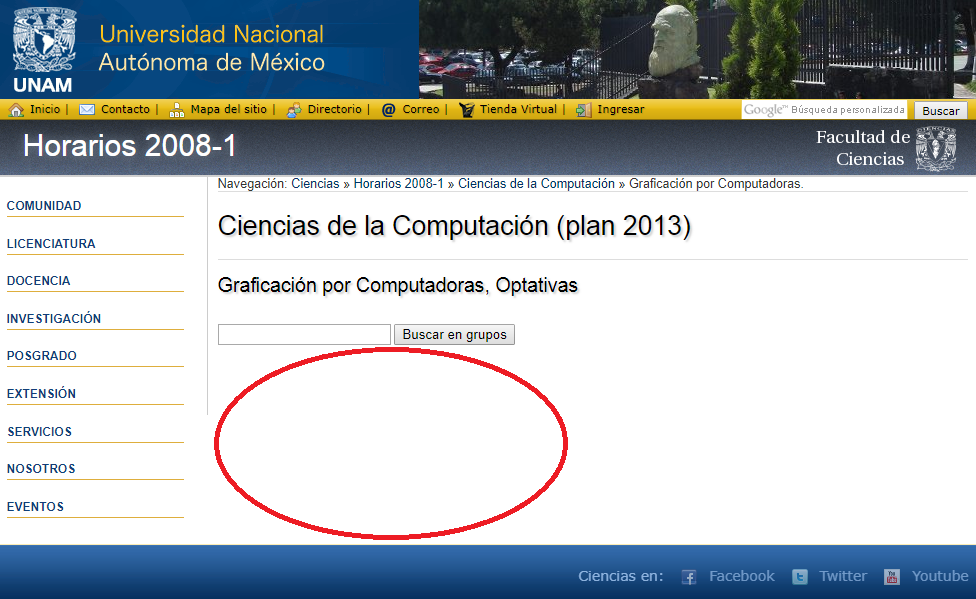
\includegraphics[scale = 0.45]{FaltaInfo_A} %width=\textwidth
\caption[\textit{Ejemplo de página web en blanco}]{\textit{Ejemplo de página web en blanco: En este tipo de páginas no encontramos información de los grupos para la materia.}}\label{pagEnBlanco}
\end{figure}

\item[-] En la figura \ref{GpoSinInfo} encontramos un ejemplo de páginas que no tienen información del salón: \url{http://www.fciencias.unam.mx/docencia/horarios/20081/119/4}

\begin{figure}[H]
\centering
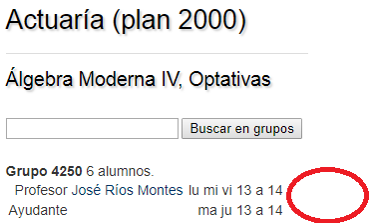
\includegraphics[scale = 0.45]{FaltaInfo_B} %width=\textwidth
\caption[\textit{Ejemplo de grupo sin información de salón}]{\textit{Ejemplo de grupo sin información de salón: En este tipo páginas no se muestra el salón en el que se imparte la clase.}}\label{GpoSinInfo}
\end{figure}

\item[-] En la figura \ref{GpoSinAlumnos} tenemos un ejemplo de páginas que tienen grupos sin información del número de alumnos inscritos en el grupo: \url{http://www.fciencias.unam.mx/docencia/horarios/20112/119/630}

\begin{figure}[H]
\centering
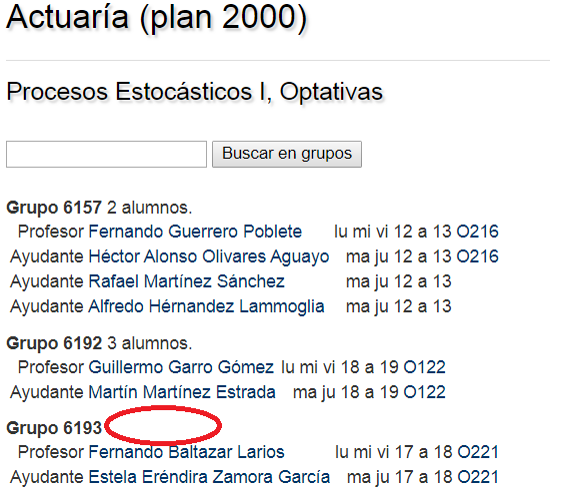
\includegraphics[scale = 0.6]{FaltaInfo_C} %width=\textwidth
\caption[\textit{Ejemplo de grupo sin información de alumnos}]{\textit{Ejemplo de grupo sin información de alumnos: En este tipo páginas encontramos grupos que no tienen el número de alumnos inscritos.}}\label{GpoSinAlumnos}
\end{figure}

\item[-] En la figura \ref{SoloHorario} vemos un ejemplo de páginas que tienen grupos sólo con el horario, sin nombre del profesor, salón, ayudante, número de alumnos, lugares disponibles: \url{http://www.fciencias.unam.mx/docencia/horarios/20091/119/841} %\url{http://www.fciencias.unam.mx/docencia/horarios/20091/119/244}

\begin{figure}[H]
\centering
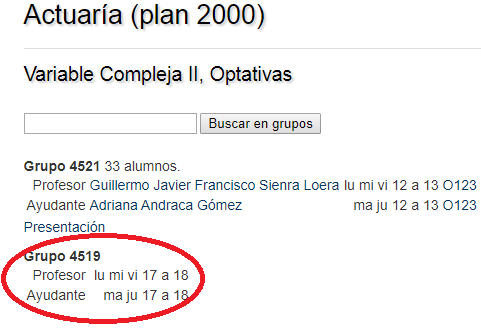
\includegraphics[scale = 0.8]{FaltaInfo_D} %width=\textwidth
\caption[\textit{Ejemplo de grupo sólo con horario}]{\textit{Ejemplo de grupo sólo con horario: En este tipo páginas existen grupos que no tienen información del profesor o salón ni del número de alumnos inscritos, sólo tienen la clave del grupo y el horario.}}\label{SoloHorario}
\end{figure}
\end{itemize} %%Subsección %%To include subfiles in to a subfiles use \input{name_of_file}
\subsection{Problemas de información repetida}

Dentro de los problemas de información repetida, encontramos diferentes casos. Para guardar la información juntamos aquellos grupos que provenían del mismo grupo. A continuación presentamos los casos que encontramos con el problema de tener información repetida.

\begin{itemize}
\item[-] En la \figurename{\ref{planRepetido}} mostramos un ejemplo en donde se tiene información de una materia correspondiente a un plan de estudios posterior al semestre en el que se está buscando la información: \url{http://www.fciencias.unam.mx/docencia/horarios/20082/1556/803} y tener la misma información con el plan de estudios correspondiente: \url{http://www.fciencias.unam.mx/docencia/horarios/20082/218/803}

El número del plan de estudios corresponde al año en que entró en vigencia el plan, por lo que no debería de existir un horario con un plan posterior al año del semestre. En la subfigura $(a)$ de la \figurename{\ref{planRepetido}} podemos ver una materia de la carrera de Ciencias de la Computación del semestre 2008-2, con el plan 2013, lo cual no es lógico. En la subfigura $(b)$ de la misma figura, vemos la infomración de la misma materia y del mismo grupo pero con el plan 1994.

\begin{figure}[H]
\centering
\subfigure[\textit{Plan de estudios posterior}]{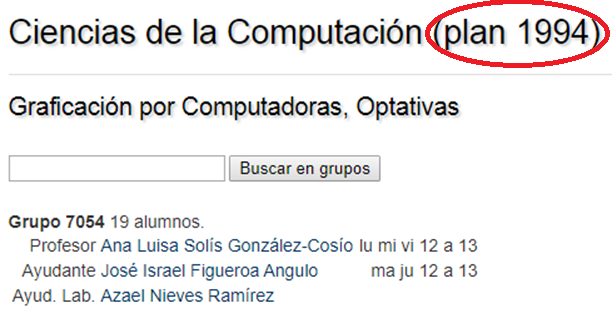
\includegraphics[width=10cm]{InfoRepetida_A_1}} %%Ping\"uino %%[angle=30]
	\subfigure[\textit{Plan de estudios correspondiente}]{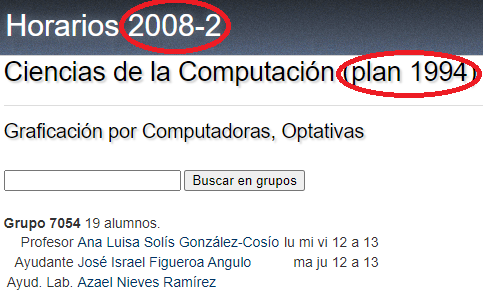
\includegraphics[width=10cm]{InfoRepetida_A_2}}
	\caption[\textit{Ejemplo de información repetida: Planes de estudio}]{\textit{Ejemplo de información repetida (Planes de estudio): No deberían de existir grupos con planes posteriores al año del semestre en el que se busca información.}}\label{planRepetido}
\end{figure}

\item[-] En la \figurename{\ref{MateriaNombresDistintos}} vemos un ejemplo en donde se tiene una misma materia con nombres distintos para las diferentes carreras: \url{http://www.fciencias.unam.mx/docencia/horarios/20201/217/1712} para Matemáicas, plan 1983 y \url{http://www.fciencias.unam.mx/docencia/horarios/20201/2017/1739} para Actuaría, plan 2015. Notamos que la información en ambas páginas es la misma, sólo cambian las claves de los grupos.

\begin{figure}[H]
	\centering
	\subfigure[\textit{Matemáticas: 1983}]{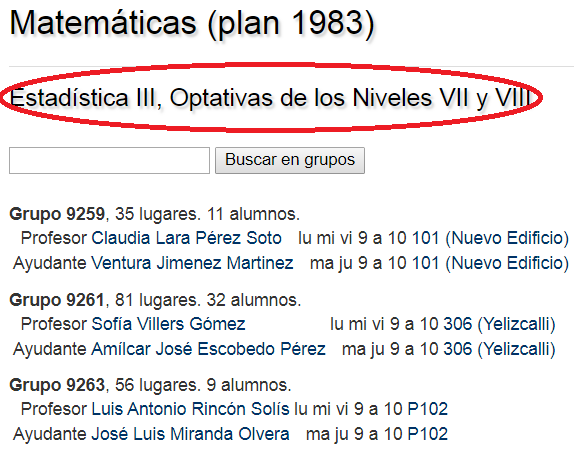
\includegraphics[width=10cm]{InfoRepetida_B_1}} %%Ping\"uino %%[angle=30]
	\subfigure[\textit{Actuaría: 2015}]{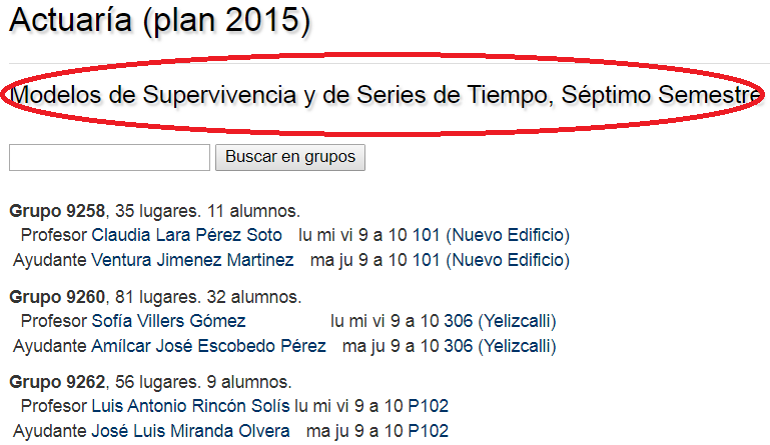
\includegraphics[width=10cm]{InfoRepetida_B_2}}
	\caption[\textit{Ejemplo de información repetida: Materia con nombres distintos}]{\textit{Ejemplo de información repetida: Materia con nombres distintos: En estos casos se tienen materias que tienen nombres diferentes de acuerdo a la carrera o plan de estudios.}}\label{MateriaNombresDistintos}
\end{figure}

\item[-] En la \figurename{\ref{UnProfMuchasMaterias}} tenemos un ejemplo de profesores que imparten dos o más clases distintas en el mismo horario y diferente salón: \url{http://www.fciencias.unam.mx/docencia/horarios/20111/2017/162} para Ecuaciones Diferenciales I y \url{http://www.fciencias.unam.mx/docencia/horarios/20111/2017/91} para Cálculo Diferencial e Integral I.
  
Las materias mencionadas son diferentes, pero las clases comienzan a la misma hora, Ecuaciones de 18-19hrs y Cálculo de 18-20hrs, dado que se tiene la misma ayudante pudiera ser que se intercambien las horas, pero no se puede asignar más de una clase a la misma hora al mismo profesor.

%EJEMPLO CON PROFESOR: Bartolo Guzmán Guevara
%Ecuaciones Diferenciales Parciales II
%\url{http://www.fciencias.unam.mx/docencia/horarios/20131/217/183}
%\url{http://www.fciencias.unam.mx/docencia/horarios/20131/119/183}
%\url{http://www.fciencias.unam.mx/docencia/horarios/20131/2055/183}
%Matemáticas Avanzadas de la Física
%\url{http://www.fciencias.unam.mx/docencia/horarios/20131/217/610}
%Funciones Especiales y Transformadas Integrales
%\url{http://www.fciencias.unam.mx/docencia/horarios/20131/218/217}
%\url{http://www.fciencias.unam.mx/docencia/horarios/20131/119/217}

%EJEMPLO CON PROFESORA: Tania Eréndira Rivera Torres. Introducción Matemática a la Mecánica Celeste y Álgebra Lineal I
%http://www.fciencias.unam.mx/docencia/horarios/20082/119/5
%http://www.fciencias.unam.mx/docencia/horarios/20082/119/356
%http://www.fciencias.unam.mx/docencia/horarios/20082/1176/5
%http://www.fciencias.unam.mx/docencia/horarios/20082/2017/5
%http://www.fciencias.unam.mx/docencia/horarios/20082/218/5
%http://www.fciencias.unam.mx/docencia/horarios/20082/1556/5
%http://www.fciencias.unam.mx/docencia/horarios/20082/217/5
%http://www.fciencias.unam.mx/docencia/horarios/20082/217/356
%http://www.fciencias.unam.mx/docencia/horarios/20082/2055/5 

%EJEMPLO CON PROFESOR: Hugo Alberto Rincón Mejía. Álgebra Moderna II y Álgebra Moderna III
%http://www.fciencias.unam.mx/docencia/horarios/20192/119/2
%http://www.fciencias.unam.mx/docencia/horarios/20081/119/3
%http://www.fciencias.unam.mx/docencia/horarios/20192/218/2
%http://www.fciencias.unam.mx/docencia/horarios/20192/1556/2
%http://www.fciencias.unam.mx/docencia/horarios/20192/217/2

%EJEMPLO CON PROFESOR: Roberto Pichardo Mendoza. Seminario de Apoyo a la Titulación en Matemáticas A y Geometría Analítica II
%http://www.fciencias.unam.mx/docencia/horarios/20192/119/245
%http://www.fciencias.unam.mx/docencia/horarios/20192/1176/245
%http://www.fciencias.unam.mx/docencia/horarios/20192/2017/245
%http://www.fciencias.unam.mx/docencia/horarios/20192/218/245
%http://www.fciencias.unam.mx/docencia/horarios/20192/217/245
%http://www.fciencias.unam.mx/docencia/horarios/20192/217/959
%http://www.fciencias.unam.mx/docencia/horarios/20192/2055/245

%EJEMPLO CON PROFESOR: Roberto Pichardo Mendoza. Seminario de Topología A y Seminario de Apoyo a la Titulación en Matemáticas A
%http://www.fciencias.unam.mx/docencia/horarios/20191/119/977
%http://www.fciencias.unam.mx/docencia/horarios/20191/217/959
%http://www.fciencias.unam.mx/docencia/horarios/20191/217/977

%EJEMPLO CON PROFESOR: Sergio Iván López Ortega. Probabilidad II y Procesos Estocásticos II
%http://www.fciencias.unam.mx/docencia/horarios/20112/119/626
%http://www.fciencias.unam.mx/docencia/horarios/20112/119/631
%http://www.fciencias.unam.mx/docencia/horarios/20112/1176/626
%http://www.fciencias.unam.mx/docencia/horarios/20112/1176/631
%http://www.fciencias.unam.mx/docencia/horarios/20112/2017/626
%http://www.fciencias.unam.mx/docencia/horarios/20112/2017/631
%http://www.fciencias.unam.mx/docencia/horarios/20112/218/626
%http://www.fciencias.unam.mx/docencia/horarios/20112/1556/626
%http://www.fciencias.unam.mx/docencia/horarios/20112/217/626
%http://www.fciencias.unam.mx/docencia/horarios/20112/217/631
%http://www.fciencias.unam.mx/docencia/horarios/20112/2055/626
%http://www.fciencias.unam.mx/docencia/horarios/20112/2055/631

%EJEMPLO CON PROFESORA: Ana Patricia Kuri González. Seminario sobre Enseñanza de las Matemáticas II y Seminario sobre Enseñanza de las Matemáticas I
%http://www.fciencias.unam.mx/docencia/horarios/20172/119/751
%http://www.fciencias.unam.mx/docencia/horarios/20172/119/754
%http://www.fciencias.unam.mx/docencia/horarios/20172/218/751
%http://www.fciencias.unam.mx/docencia/horarios/20172/218/754
%http://www.fciencias.unam.mx/docencia/horarios/20172/217/751
%http://www.fciencias.unam.mx/docencia/horarios/20172/217/754

%EJEMPLO CON PROFESORA: Tania Eréndira Rivera Torres. Introducción Matemática a la Mecánica Celeste y Álgebra Lineal I
%http://www.fciencias.unam.mx/docencia/horarios/20082/119/5
%http://www.fciencias.unam.mx/docencia/horarios/20082/119/356
%http://www.fciencias.unam.mx/docencia/horarios/20082/1176/5
%http://www.fciencias.unam.mx/docencia/horarios/20082/2017/5
%http://www.fciencias.unam.mx/docencia/horarios/20082/218/5
%http://www.fciencias.unam.mx/docencia/horarios/20082/1556/5
%http://www.fciencias.unam.mx/docencia/horarios/20082/217/5
%http://www.fciencias.unam.mx/docencia/horarios/20082/217/356
%http://www.fciencias.unam.mx/docencia/horarios/20082/2055/5

%EJEMPLO CON PROFESOR: Juan Rivera Alcántara. Teoría del Riesgo y Valuación de Opciones
%http://www.fciencias.unam.mx/docencia/horarios/20082/119/1067
%http://www.fciencias.unam.mx/docencia/horarios/20082/119/1807
%http://www.fciencias.unam.mx/docencia/horarios/20082/1176/1067
%http://www.fciencias.unam.mx/docencia/horarios/20082/1176/1807
%http://www.fciencias.unam.mx/docencia/horarios/20082/2017/1807

%EJEMPLO CON PROFESOR: Javier Valdez Quijada. Teoría de los Números I y Teoría de los Números II
%http://www.fciencias.unam.mx/docencia/horarios/20172/119/764
%http://www.fciencias.unam.mx/docencia/horarios/20172/119/777
%http://www.fciencias.unam.mx/docencia/horarios/20172/218/764
%http://www.fciencias.unam.mx/docencia/horarios/20172/218/777
%http://www.fciencias.unam.mx/docencia/horarios/20172/1556/764
%http://www.fciencias.unam.mx/docencia/horarios/20172/1556/777
%http://www.fciencias.unam.mx/docencia/horarios/20172/217/764
%http://www.fciencias.unam.mx/docencia/horarios/20172/217/777



%EJEMPLO CON PROFESOR: 
%EJEMPLO CON PROFESORA: 


\begin{figure}[H]
	\centering
	\subfigure[\textit{Ecuaciones Diferenciales I}]{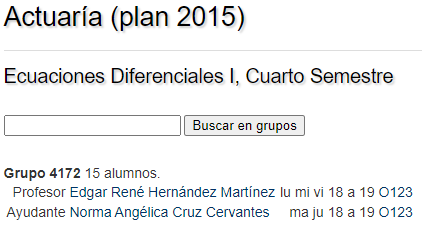
\includegraphics[width=10cm]{Ej_gpo_repetido_1}} %%Ping\"uino %%[angle=30]
	\subfigure[\textit{Cálculo Diferencial e Integral I}]{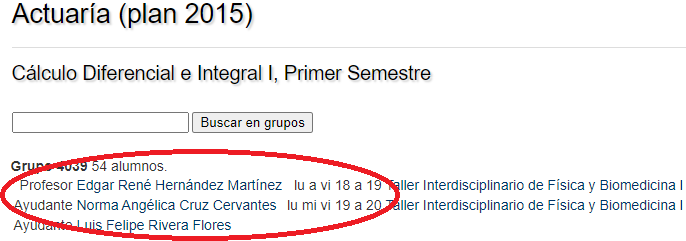
\includegraphics[width=15cm]{Ej_gpo_repetido_2}}
	\caption[\textit{Ejemplo de información repetida: Mismo profesor, materias distintas}]{\textit{Ejemplo de información repetida (mismo profesor, materias distintas): En este caso se tiene más de una clase impartida por el mismo profesor a la misma hora en diferente salón lo cual no debería de ocurrir.}}\label{UnProfMuchasMaterias}
\end{figure}	

\end{itemize}
 %%Subsección
\subsection{Otros problemas al extraer información}

En algunos de los problemas que surgieron, encontramos detalles particulares que tuvimos que resolver caso por caso. Ésto para poder guardar la información de manera adecuada. A continuación se presentan los diferentes casos encontrados:

  \begin{itemize}
\item[-] Dentro de la obtención de datos del número de alumnos, no se lee la información cuando se tiene \textit{Un alumno}, ya que no se reconoce el texto \textit{Un} como el número $1$. En la \figurename{~\ref{UnAlumno}} vemos un ejemplo de este caso.

\begin{figure}[H]
\centering
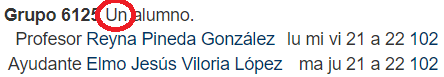
\includegraphics[scale = 0.8]{Ej_un_alumno} %width=\textwidth
%\url{http://www.fciencias.unam.mx/docencia/horarios/20081/119/1809}
\caption[\textit{Ejemplo de grupo con un alumno}]{\textit{Ejemplo de grupo con un alumno: En este caso se tiene el texto ``Un'' y no un número ``1''.}}\label{UnAlumno}
\end{figure}

Para resolver este problema se identificó la variable tipo \textit{string} igual a \textit{Un} para convertir la información y así poder utilizar los datos obtenidos.

\item[-] El algoritmo supone que todas las clases duran una hora y no se consideran las medias horas: \url{http://www.fciencias.unam.mx/docencia/horarios/20172/1556/820}. En la \figurename{~\ref{MediasHoras}} mostramos un ejemplo en donde se considera que esa materia inicia a las 18hrs.

\begin{figure}[H]
\centering
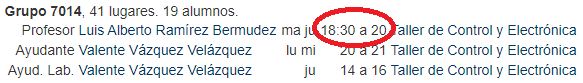
\includegraphics[scale = 0.9]{Ej_gpo_medias_hrs} %width=\textwidth
%\url{http://www.fciencias.unam.mx/docencia/horarios/20172/1556/820}
\caption[\textit{Ejemplo de grupo con medias horas}]{\textit{Ejemplo de grupo con medias horas: Se considera que las materias inician en horas enteras y no a las medias horas.}}\label{MediasHoras}
\end{figure}

\item[-] Se tienen materias con múltiples horarios: \url{http://www.fciencias.unam.mx/docencia/horarios/20181/2055/1323}. En estos casos sólo se registran los horarios y salones en los que los profesores imparten su clase, no se toman en cuenta las clases impartidas por los ayudantes.

En la \figurename{~\ref{horariosMultiples}} tenemos un ejemplo de este caso en donde el profesor imparte su clase los lunes, miércoles y viernes de 13-14hrs en el salón O215, hay una ayudantía los martes y jueves de 13-14hrs en el salón O215 y otra ayudantía los martes de 11-13hrs en el salón 304 (Yelizcalli). Se considera que esta materia inicia a las 13hrs y se imparte en el salón O215.

\begin{figure}[H]
\centering
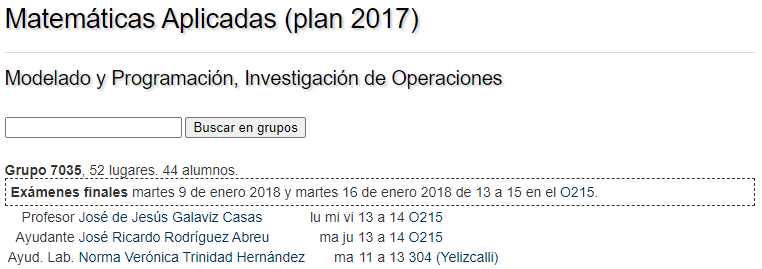
\includegraphics[scale = 0.8]{Ej_gpo_horarios_multiples} %width=\textwidth
\caption[\textit{Ejemplo de grupo con horarios múltiples}]{\textit{Ejemplo de grupo con horarios múltiples: En estos grupos sólo se toman en cuenta los horarios y salones en los que los profesores imparten clase.}}\label{horariosMultiples}
\end{figure}

\item[-] Las materias de inglés no se imparten todos los días de la semana, en algunos casos se imparten clases en línea: \url{http://www.fciencias.unam.mx/docencia/horarios/20202/2017/1135}. Se registran únicamente los horarios de los días en que se imparten las clases presenciales. En la \figurename{~\ref{casoIngles}} mostramos un ejemplo de este caso.

\begin{figure}[H]
\centering

\includegraphics[scale = 1]{Ej_gpo_ingles} %width=\textwidth
\caption[\textit{Ejemplo de grupo de inglés}]{\textit{Ejemplo de grupo de inglés: Las clases no se imparten todos los días. Hay sesiones virtuales. Sólo se toma en cuenta el horario de las clases presenciales.}}\label{casoIngles}
\end{figure}

\item[-] Se tienen grupos que no tienen la misma estructura que los tipos de grupos \textbf{A}, \textbf{B} y \textbf{C} definidos en la Sección \ref{TiposDeGpos}: \url{http://www.fciencias.unam.mx/docencia/horarios/20201/2017/872}, debido a ello el código CSS utilizado no sirve para obtener toda la información que se puede obtener del grupo. En la \figurename{~\ref{GpoEstructuraDiferente}} tenemos un ejemplo de este caso en donde no se lee adecuadamente el número de alumnos inscritos en el grupo.

\begin{figure}[H]
\centering
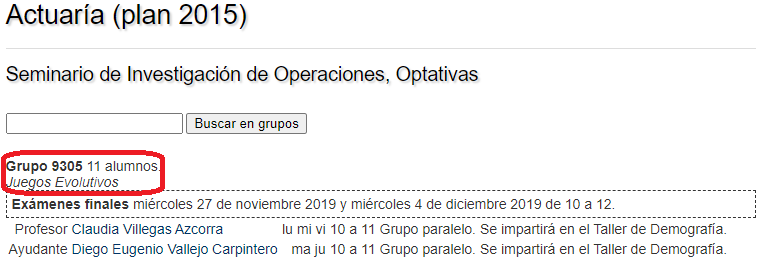
\includegraphics[scale = 0.8]{Ej_gpo_con_estructura_diferente} %width=\textwidth
\caption[\textit{Ejemplo de grupo con estructura diferente}]{\textit{Ejemplo de grupo con estructura diferente: En estos casos no se extrae adecuadamente la información de los grupos porque el código CSS utilizado no corresponde a este tipo de grupos.}}\label{GpoEstructuraDiferente}
\end{figure}

\end{itemize} %%Subsección

\section{Matrices de datos}

Una vez que se realizó el proceso de la limpieza de los datos obtenidos, éstos se guardaron, por semestre, en matrices llamadas \textit{m\_grande}. Los nombres de sus columnas con su respectiva explicación y posibles valores, se muestran en la siguiente tabla:

\dfNmatrizGrande %%Tabla con la información de la matriz grande

La columna \textit{Cambios}, va a guardar todos los cambios que ha tenido cada grupo. El significado de los números que pueden aparecer en esa columna se explican a continuación:

\begin{enumerate}
\item[(1)] Grupos con detalles particulares.

\item[(2)] Se anotaron los días en los que se imparte la materia, en la columna \textit{Horario}, por ejemplo cuando había conflicto debido a que el profesor impartía más de una materia a la misma hora, al revisar el caso se encontró que los días en los que se impartía la clase era distinto.

\item[(3)] Se eliminaron los grupos repetidos, al juntar la información en un mismo grupo.

\item[(4)] Páginas que no tienen información del salón.

\item[(5)] Actualización del número de materia por cambio de nombre o agrupamiento de materias.
\end{enumerate}
